\chapter{Extraction Pipeline}

\section{Motivation and Objective}
Extracting accurate, structured information from historical documents presents a distinct set of challenges. Primary difficulties include scanning noise and complex page layouts, such as fading ink, skew, and dense multi-column formatting. In this context, the central question is how to obtain \emph{structured} outputs (e.g., TSV/JSON) while remaining faithful to the evidence present on the page.

To motivate our design choices, we compare four extraction paradigms that represent the main families of practical approaches for this task:
\begin{enumerate}
    \item Traditional OCR
    \item Multimodal LLM (image input)
    \item Multimodal LLM (image + traditional OCR output)
    \item Text-only LLM (traditional OCR input)
\end{enumerate}

\section{Comparison of Four Extraction Methods}
\subsection{Method 1: Traditional OCR}
Traditional OCR engines are designed for faithful character-level transcription from document images. In this setting, they offer a strong form of grounding: every output token is directly tied to observed glyphs.
However, they lack semantic and layout reasoning. When glyphs are unclear or layouts are intricate, their performance degrades significantly, leading to typical failure modes such as:
\begin{itemize}
    \item \textbf{Layout entanglement:} merging distinct entries or mixing details from adjacent columns.
    \item \textbf{Noise sensitivity:} misrecognizing stains or unwanted decorative symbols
    \item \textbf{Schema mismatch:} producing text that is not naturally aligned with the desired structured format.
\end{itemize}
As a result, OCR alone could be used for transcription yet unreliable for \emph{record-level} extraction.

\subsection{Method 2: Multimodal LLM (Image Input Only)}
A multimodal LLM can directly map the document image to structured outputs, often producing clean and well-formatted results even in the presence of layout complexity. This approach is attractive because the model can jointly reason about visual layout and semantic content.
Nevertheless, it suffers from a crucial limitation: the lack of explicit grounding constraints. The model may \textbf{hallucinate} or \textbf{over-correct}, for example:
 replacing uncertain glyphs with plausible but incorrect names, dates, or addresses.
In historical documents where uncertainty is frequent, such unconstrained generation can be costly.

\subsection{Method 3: Multimodal LLM (Image + OCR Output)}
A common mitigation is to provide the multimodal LLM with both the image and the traditional OCR transcription. Intuitively, the OCR text can serve as an additional evidence channel that encourage the model toward fidelity, while the image preserves access to layout cues and hard-to-recognize regions.
This hybrid setup often improves robustness, but it raises cost as it is using both textual and image input.

\subsection{Method 4: Text-only LLM (OCR Input Only)}
As is shown in Figure~\ref{fig:extraction_pipeline}, an alternative is to restrict the LLM to \emph{text-only} processing by feeding it the OCR transcription (and a target schema) while withholding the image. In this design, the OCR output becomes the sole evidence source, and the LLM is tasked with transforming an imperfect transcription into a structured representation.
Concretely, the LLM can play two constrained roles:
\begin{enumerate}
    \item \textbf{Noise filtering:} identifying and removing non-entry content (e.g., advertisements) and OCR artifacts.
    \item \textbf{Schema alignment:} segmenting, labeling, and formatting the remaining text into TSV/JSON records.
\end{enumerate}
Because the model cannot access visual signals, it has fewer opportunities to introduce visually-motivated ``guesses.'' However, lack of visual information could also limit the accuracy of annotation, especially when the input OCR text is too noisy.

\section{Summary of Trade-offs}
The four methods have different trade-offs for \textbf{fidelity to observed evidence} and \textbf{ability to resolve layout/semantic ambiguity}:
\begin{itemize}
    \item \textbf{Traditional OCR} emphasizes character-level faithfulness but struggles with structure in complex layouts.
    \item \textbf{Multimodal LLM (image only)} emphasizes end-to-end structuring but risks hallucination and over-correction.
    \item \textbf{Multimodal LLM (image + OCR)} adds an evidence anchor yet cost more.
    \item \textbf{Text-only LLM (OCR only)} prioritizes evidence-constrained restructuring, but also constrained by the quality of OCR text.
\end{itemize}

Since each method has its own advantages and drawbacks, it's important to evaluate them in concrete application scenarios, in order to find out which works best in our task.


\begin{figure}[htbp]
    \centering
    % RESIZEBOX: This forces the image to fit the page width
    \resizebox{\textwidth}{!}{%
    
    \begin{tikzpicture}[
        % REDUCED DISTANCES: Tighter spacing between nodes
        node distance=0.6cm and 0.8cm,
        % COMPACT STYLES
        process/.style={
            rectangle, 
            rounded corners, 
            draw=blue!70!black, 
            fill=blue!5, 
            thick, 
            minimum height=1.2cm, 
            text width=2.2cm, % Made narrower
            align=center, 
            drop shadow,
            font=\small % Smaller font
        },
        data/.style={
            trapezium, 
            trapezium left angle=70, 
            trapezium right angle=110, 
            draw=orange!70!black, 
            fill=orange!5, 
            thick, 
            minimum height=1.2cm, 
            text width=2cm, % Made narrower
            align=center,
            inner sep=4pt,
            font=\small
        },
        input/.style={
            rectangle, 
            draw=gray!60!black, 
            dashed, 
            fill=gray!5, 
            minimum height=0.8cm, 
            text width=2cm, 
            align=center,
            font=\footnotesize
        },
        arrow/.style={
            -{Latex[length=2.5mm]}, 
            thick, 
            draw=gray!70!black
        },
        label/.style={
            font=\scriptsize\itshape, % Smaller label font
            text=gray!80!black,
            align=center
        }
    ]

    % --- Nodes ---

    % 1. Input Image
    \node[data] (img) {Document Page (Image)};
    \node[label, below=0.1cm of img] (img_desc) {Noise, Skew,\\Layouts};

    % 2. Process: OCR
    \node[process, right=of img] (ocr) {\textbf{Traditional OCR}};

    % 3. Intermediate: Raw Text
    \node[data, right=of ocr] (raw) {Raw\\Transcription};
    \node[label, below=0.1cm of raw] (raw_desc) {Textual Anchor};

    % 4. Process: LLM
    \node[process, right=of raw] (llm) {\textbf{Text LLM}\\(Correction)};

    % 5. Output: Structured Data
    \node[data, right=of llm] (output) {Structured\\Data};
    \node[label, below=0.1cm of output] (data_desc) {Clean, structured tsv data};
    
    % 6. External Input: Schema
    \node[input, above=0.5cm of llm] (schema) {Prompt};

    % --- Arrows ---
    \draw[arrow] (img) -- (ocr);
    \draw[arrow] (ocr) -- (raw);
    \draw[arrow] (raw) -- (llm);
    \draw[arrow] (llm) -- (output);
    \draw[arrow] (schema) -- (llm);

    % --- Background Box ---
    \draw[dashed, gray!40, rounded corners] 
        ($(img.north west)+(-1.5, 1.5)$) rectangle ($(output.south east)+(1.5, -1.5)$);
    \node[anchor=north west, text=gray!60, font=\bfseries\footnotesize] at ($(img.north west)+(-0.2, 1.2)$) {Two Stage Extraction Pipeline};

    \end{tikzpicture}
    } % End of resizebox
    
    \caption{The two-stage extraction pipeline. Traditional OCR creates a textual anchor, which the LLM structures according to the prompt.}
    \label{fig:extraction_pipeline}
\end{figure}

\section{Evaluation}
\label{sec:evaluation}

In this section, we conduct a series of experiments to validate the effectiveness of our approach. Specifically, we aim to address the following research questions (RQs):


\begin{enumerate}
    \item \textbf{RQ1:} Which data source should we use for the extraction?
    \item \textbf{RQ2:} Which model should we use for the extraction?
\end{enumerate}


\subsection{Dataset}
Our evaluation benchmark consists of a curated set of historical documents (30 pages) created in the previous section. 



\subsection{Experimental Setup}

\paragraph{Model Selection}
For the generative components, we evaluate 4 state-of-the-art Large Language Models: \textbf{GPT-5.2} and \textbf{Gemini 3 Pro} and their light version \textbf{GPT-5 mini} and \textbf{Gemini 3 Flash}. For the initial text recognition layer, we utilize two sources: the open-source \textbf{Tesseract} engine and the legacy OCR metadata provided with the \textit{Guide Rosenwald} digitization.

\paragraph{Baselines and Comparisons}
To validate the effectiveness of our extraction strategy, we compare four representative methods below:

\begin{enumerate}
    \item \textbf{Traditional OCR:} Direct use of OCR transcriptions (Tesseract and the existing \textit{Guide Rosenwald} OCR) without any LLM-based post-processing.
    \item \textbf{Multimodal LLM (Image Only):} End-to-end extraction that maps an image crop directly to structured output using a vision-language model, without providing the OCR transcription.
    \item \textbf{Multimodal LLM (Image + OCR):} A hybrid setup in which the vision-language model receives both the image crop and the OCR transcription, allowing it to leverage visual cues while being guided by textual evidence.
    \item \textbf{Text-only LLM (OCR Only):} A two-stage configuration, where a text LLM receives only the OCR transcription (with a target schema) and is used solely for noise filtering and schema alignment, treating OCR as the sole evidence source.
\end{enumerate}


\section{Quantitative Analysis}
\begin{table}[htbp]
\centering
\small
\setlength{\tabcolsep}{6pt}
\renewcommand{\arraystretch}{1.2}
\begin{tabular}{llrrrr}
\toprule
\textbf{Source} & \textbf{Model} & \textbf{Avg WER} & \textbf{Mid WER} & \textbf{Avg CER} & \textbf{Mid CER} \\
\midrule
\multirow{4}{*}{Image + Original OCR}
 & \texttt{gemini-3-pro-preview}    & \textbf{0.0360} & \textbf{0.0293} & \textbf{0.0139} & \textbf{0.0088} \\
 & \texttt{gemini-3-flash-preview}  & \underline{0.0435} & \underline{0.0403} & \underline{0.0177} & \underline{0.0108} \\
 & \texttt{gpt-5.2-2025-12-11}      & 0.0581 & 0.0543 & 0.0178 & 0.0149 \\
 & \texttt{gpt-5-mini-2025-08-07}   & 0.1026 & 0.0645 & 0.0581 & 0.0192 \\
\midrule
\multirow{4}{*}{Image}
 & \texttt{gemini-3-pro-preview}    & \textbf{0.0372} & \textbf{0.0347} & \textbf{0.0143} & \textbf{0.0092} \\
 & \texttt{gemini-3-flash-preview}  & \underline{0.0413} & \underline{0.0355} & \underline{0.0167} & \underline{0.0106} \\
 & \texttt{gpt-5.2-2025-12-11}      & 0.2024 & 0.1133 & 0.1405 & 0.0384 \\
 & \texttt{gpt-5-mini-2025-08-07}   & 0.1274 & 0.0877 & 0.0650 & 0.0327 \\
\midrule
\multirow{5}{*}{Original OCR}
 & \texttt{gemini-3-pro-preview}    & \textbf{0.0959} & \textbf{0.0751} & \underline{0.0373} & \textbf{0.0264} \\
 & \texttt{gemini-3-flash-preview}  & \underline{0.0989} & 0.0910 & \textbf{0.0314} & \underline{0.0292} \\
 & \texttt{gpt-5.2-2025-12-11}      & 0.1132 & \underline{0.0794} & 0.0415 & 0.0317 \\
 & \texttt{gpt-5-mini-2025-08-07}   & 0.1580 & 0.1155 & 0.0701 & 0.0471 \\
 & \texttt{raw\_ocr}                & 0.3948 & 0.3257 & 0.1862 & 0.0998 \\
\midrule
\multirow{5}{*}{Tesseract OCR}
 & \texttt{gemini-3-pro-preview}    & \underline{0.2405} & 0.1681 & \underline{0.1592} & \underline{0.0667} \\
 & \texttt{gemini-3-flash-preview}  & \textbf{0.1618} & \textbf{0.1267} & \textbf{0.0890} & \textbf{0.0475} \\
 & \texttt{gpt-5.2-2025-12-11}      & 0.2644 & \underline{0.1566} & 0.1838 & 0.0709 \\
 & \texttt{gpt-5-mini-2025-08-07}   & 0.3230 & 0.2378 & 0.2246 & 0.1068 \\
 & \texttt{raw\_ocr}                & 0.8387 & 0.5956 & 0.4594 & 0.3611 \\
\bottomrule
\end{tabular}
\caption{OCR and post-OCR correction performance across sources and models (30 documents). The best result of each source is bold, and the second best is underlined. (Avg is the macro avg over files)}
\label{tab:ocr_results_30docs}
\end{table}
\begin{figure}
    \centering
    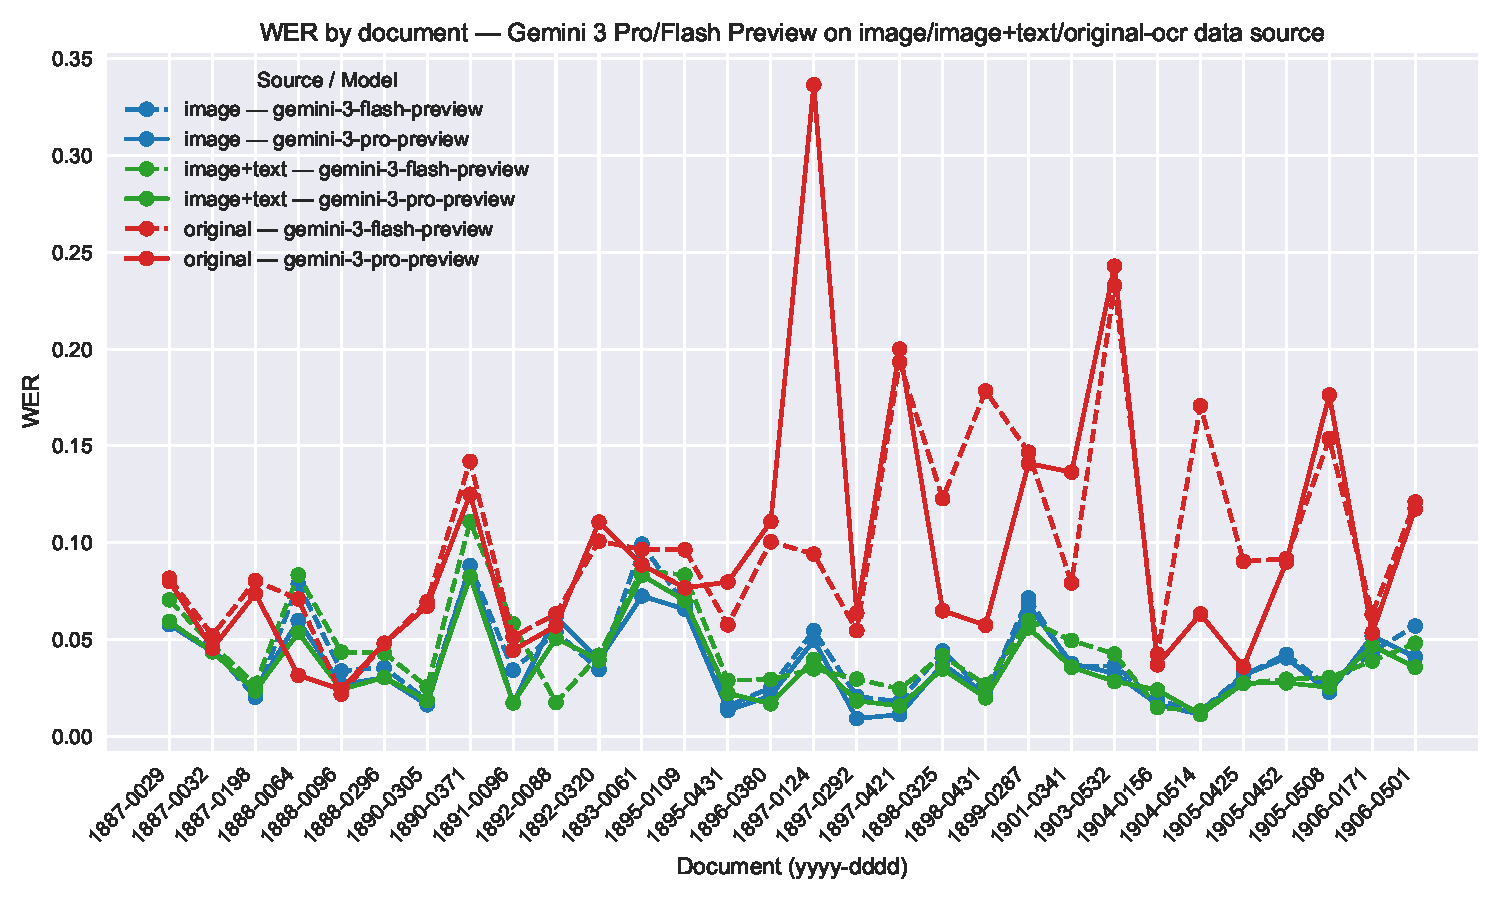
\includegraphics[width=\linewidth]{Images/gemini3pro_flash_wer_by_source.pdf}
    \caption{WER by document (Gemini 3 family)}
    \label{fig:model_to_use}
    \footnotesize{('1899', '0287'), ('1903', '0532') these two years do not have original OCR, using Tesseract OCR instead}
\end{figure}


\subsection{RQ1: Which data source should we use for the extraction?}

Table ~\ref{tab:ocr_results_30docs} shows the Word Error Rate (WER) and Character Error Rate (CER) across all the models and data sources. By comparing the best-performing (bolded) results across all data sources, we observe that \emph{Image + Original OCR} consistently achieves the lowest error rate on all metrics, followed by \emph{Image} alone. Both image-based settings show a substantial lead over \emph{Original OCR} and \emph{Tesseract OCR}. However, in Figure~\ref{fig:model_to_use}, while the WER of Original (text only LLM with Original-OCR input) is usually higher than image and image+text source, there are exceptions in 1888-0064 and 1888-0096.



These results indicate that the quality of the input data source is the primary factor influencing extraction performance. The image modality contains the most complete and faithful information, and starting directly from images leads to strong results, especially given the capabilities of current multimodal LLMs. Augmenting images with the original OCR text can further improve accuracy, as the textual signal may help disambiguate certain fields and reduce model uncertainty.

In contrast, when relying solely on OCR outputs (either original or Tesseract) without access to images, the LLM functions mainly as a post-correction mechanism. In such cases, extraction quality is strongly constrained by the underlying OCR quality. For example, Tesseract OCR produces noisier text than the original OCR, its downstream extraction and post-correction performance degrades accordingly.

In summary, images should be included in the input for extraction. Adding the original OCR as auxiliary information provides modest additional gains. The final choice between \emph{Image} and \emph{Image + Original OCR} should be informed by further analysis using more fine-grained, field-level metrics rather than relying solely on aggregate performance measures, since the metric difference is small between these two sources.

\subsection{RQ2: Which model should we use for the extraction?}

Table ~\ref{tab:ocr_results_30docs} shows that across both the \emph{Image} and \emph{Image + Original OCR} settings, \texttt{gemini-3-pro-preview} consistently achieves the best performance, followed closely by \texttt{gemini-3-flash-preview}. This highlights the strong overall capability of the Gemini~3 family for our extraction task.

At the same time, the performance gap between the Pro and Flash variants remains relatively small, and the advantage of the Pro model is not always consistent across all the files (see Figure~\ref{fig:model_to_use}). This suggests that lighter models, which offer substantially lower latency and cost, are already capable of delivering competitive extraction quality in this scenario.

Consequently, while \texttt{gemini-3-pro-preview} represents overall higher accuracy, \texttt{gemini-3-flash-preview} constitutes a compelling alternative when efficiency considerations are prioritized. The final model choice should therefore balance marginal accuracy gains against computational cost and throughput requirements.

\subsection{Summary of Quantitative Analysis}
From the quantitative analysis above, to pick the best strategy for our extraction, we can narrow down our choices to:
\begin{enumerate}
    \item Model: Gemini 3 Pro Preview or Gemini 3 Flash Preview
    \item Source: Image + Text or Image only
\end{enumerate}
Since these four combinations exhibit comparable performance, we further rely on qualitative analysis to differentiate them and identify the most suitable strategy. In addition, the text-only LLM with original OCR input is also included in the qualitative analysis. This model served as our primary approach in the initial studies, and its inclusion provides a complementary perspective on text-only post-correction performance.


\section{Qualitative Analysis}
In this section, we conduct a qualitative, file-level analysis to examine representative cases in which the word and character error rates differ across model–input combinations. Rather than focusing on aggregate metrics, we inspect individual files to understand the nature of errors, the conditions under which error rates increase or decrease, and whether these behaviors are consistent with the overall quantitative results.

\begin{enumerate}
    \item \textbf{1897-0124}: In case of error rate,
    \textit{Image+Text Gemini~3~Pro} $<$ \textit{Image Gemini~3~Pro} $<$ \textit{Original OCR + Gemini~3~Flash Preview} $<$ \textit{Original OCR + Gemini~3~Pro Preview}.  
    The first inequality is consistent with the global evaluation results. However, the latter comparison is unexpected from a model-capacity perspective, as the Pro variant performs worse than the Flash model under identical original OCR input.

    % \item \textbf{1905-0452}: Image+Text Gemini~3~Pro $<$ Image Gemini~3~Pro
    % \item \textbf{1891-0096}: Image+Text Gemini~3~Pro $<$ Image Gemini~3~Pro

    \item \textbf{1904-0514}: \textit{Image+Text Gemini~3~Pro}, \textit{Image Gemini~3~Pro} $<$ \textit{Original OCR + Gemini~3~Pro Preview}. 
    A case in which only the text-only pipeline with original OCR input produces a high error rate, while all image-based or image+text configurations perform reliably. This file highlights the limitations of post-correction without visual grounding.

    \item \textbf{1893-0061}: 
    \textit{Image Gemini~3~Pro} $<$ \textit{Image+Text Gemini~3~Pro}, contradicting the overall trend in which multimodal input generally yields lower error rates. This case motivates a closer inspection of how auxiliary textual input may introduce noise.
\end{enumerate}
% \section{Qualitative Analysis}

% Here we are going to focus on several specific files, to see the details of error rate, how they are high or low. 

% \begin{enumerate}
%     \item 1897-0124, image+text gemini3 pro < image gemini 3 pro < original gemini 3 flash preview < original gemini 3 pro preview. The first < is aligned with the overall results but the last < is not expected from the model capacity perspective.
%     % \item 1905-0452 image+text gemini 3 pro < image gemini 3 pro
%     % \item 1891-0096 image+text gemini 3 pro < image gemini 3 pro
%     \item 1904-0514 why only original ocr text input fails
%     \item 1893-0061 image gemini 3 pro < image+text gemini 3 pro, contrary to the overall results
% \end{enumerate}

\subsection{1897-0124}

\subsubsection{Why Image + Text wins over Image Only}
Figure~\ref{fig:1897_0124_image} shows the entries in page 1897-0124. Table~\ref{tab:model_comparison_errors} shows two examples where Image + Text input outperforms Image only input in this image. In the first example, with Image Only, the model recognizes the year as 1868, while in the image it shows 1868. In raw OCR text (original OCR), it shows 1868, and with Image + Text input, the model outputs the correct year. With Original OCR only, the model also outputs the correct result. This shows that Image Only input method could be unstable on certain points, and additional Text information could help the correction.

\begin{table}[htbp]
\centering
\small
\begin{tabular}{llll}
\hline
\textbf{Source} & \textbf{Name} & \textbf{Year} & \textbf{Address} \\
\hline
REF & viégarnier & 1868 & av des ternes 63 \\
Image + Text & viégarnier & 1868 & av des ternes 63 \\
Image Only & viégarnier & \textcolor{red}{1866} & av des ternes 63 \\
Original OCR Only & viégarnier & 1868 & av des ternes 63 \\
Raw OCR & viégarnier & 1868 & av \textcolor{red}{dès} ternes 63 \\
\hline
REF & vigoureux & 1868 & vaugirard 33 \\
Image + Text & vigoureux & 1868 & vaugirard 33 \\
Image Only & \textcolor{red}{vigouretix} & 1868 & vaugirard 33 \\
Original OCR Only & vigoureux & 1868 & vaugirard 33 \\
Raw OCR & \textcolor{red}{viçfoureux} & \textcolor{red}{186s} & vaugirard 33 \\
\hline
\end{tabular}
\caption{Gemini 3 Pro Preview outputs compared to ground truth (REF). Errors are highlighted in red.}
\label{tab:model_comparison_errors}
\end{table}

In addition, in the raw OCR, the "des" in the address is recognized as "dès". Although "dès" is a valid French word, it is not grammatically and semantically correct here. Image Only, Image + Text and Original OCR Only model corrected this error, showing the capability of semantic correction, or the usability of LLM prior knowledge in our correction task.

In the second example, with Image Only, the model has a wrong recognition on the name. The raw OCR also made mistakes on the name, which however reserves the correct suffix "reux", which could be a common suffix in French words. With Image + Text input, and Original OCR Only input, our model successfully corrected this error. One possible explanation is that vigoureux is a common French word and also a possible surname. This word is recognized by our model through its prior knowledge. This once more shows the unstability of Image Only input method.

When it comes to the year, the raw OCR has the year 1868 recognized as 186s, which is not a valid year. It's acceptable for the OCR because it only follows the string as it is, rather than cooperating semantic knowledge. All of our input modalities, corrected this mistake, again showing the capability of semantic correction.




\begin{figure}
    \centering
    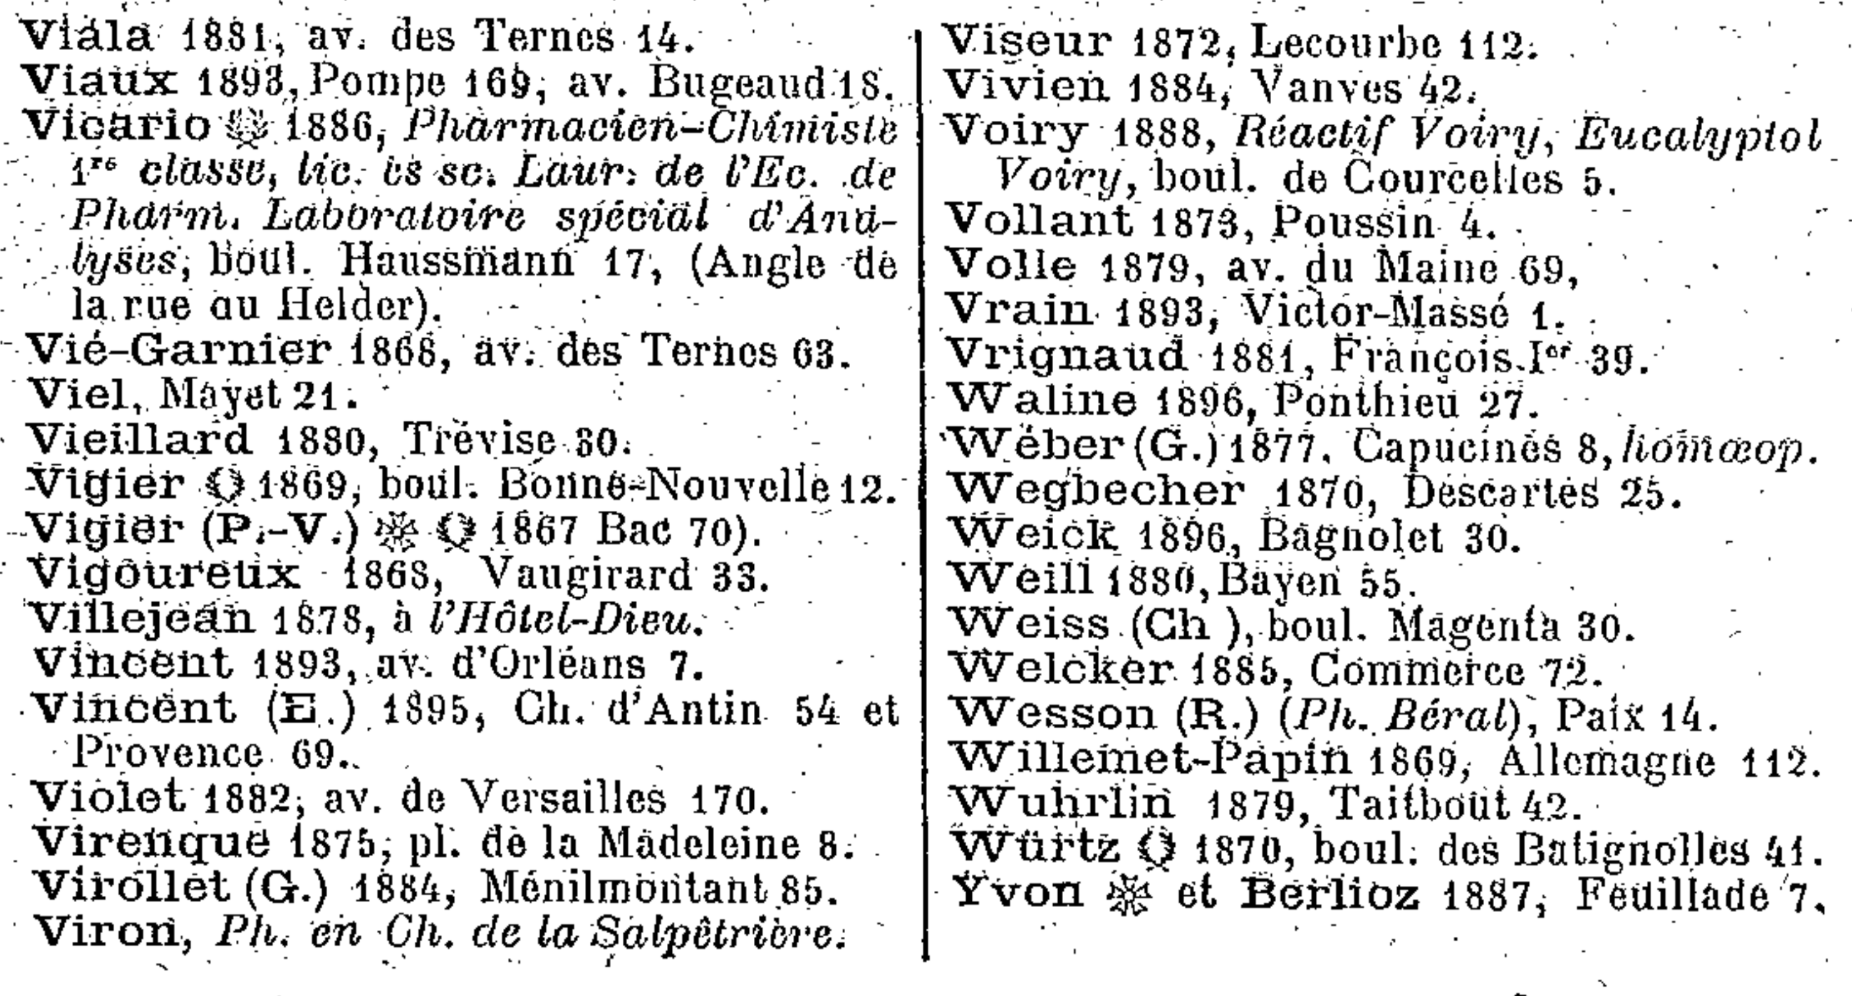
\includegraphics[width=0.8\linewidth]{Images/1897-0124.png}
    \caption{1897-0124 image}
    \label{fig:1897_0124_image}
\end{figure}

\subsubsection{Why pro fails flash}

\begin{table}
\centering
\small
\renewcommand{\arraystretch}{1.2}
\begin{tabularx}{\linewidth}{lX}
\hline
\textbf{Source} & \textbf{Transcription} \\
\hline

REF &
vicario 1886 pharmacien-chimiste 1re classe lic ès sc laur de l'ec de pharm laboratoire spécial d'analyses
boul haussmann 17 angle de la rue au helder \\

Gemini 3 Flash Preview &
\textcolor{red}{vibario} 1886 pharmacien-chimiste 1re classe lic ès sc laur de l'ec de pharm laboratoire spécial d'analyses
boul haussmann 17 angle de la rue au helder \\

Gemini 3 Pro Preview &
\textcolor{red}{[entry missed completely]} \\

Raw OCR &
\textcolor{red}{vibàrio sjï886 phàrmaciencmviislé classe lie bs se laur~ de vec de pharm}
laboratoire spécial \textcolor{red}{dana lyses}
boul \textcolor{red}{haussiïiânn} 17 angle \textcolor{red}{dé larue} au helder \\

\hline

REF &
viron \textcolor{red}{phu} en ch de la salpêtrière \\

Gemini 3 Flash Preview &
viron ph en ch de la salpêtrière \\

Gemini 3 Pro Preview &
\textcolor{red}{[entry missed completely]} \\

Raw OCR &
\textcolor{red}{viroh} ph \textcolor{red}{eh gh} de lasàlpùtriere \\

\hline

REF &
voiry 1888 réactif voiry eucalyptol voiry boul de courcelles 5 \\

Gemini 3 Flash Preview &
voiry 1888 réactif voiry eucalyptol voiry boul de courcelles 5 \\

Gemini 3 Pro Preview &
\textcolor{red}{[entry missed completely]} \\

Raw OCR &
voiry 1888 réactif voiry \textcolor{red}{èucalypiol} voiry
boul de \textcolor{red}{courceiles} 5 \\

\hline

REF &
wesson r ph béral paix 14 \\

Gemini 3 Flash Preview &
wesson r ph béral paix 14 \\

Gemini 3 Pro Preview &
\textcolor{red}{[entry missed completely]} \\

Raw OCR &
wesson r \textcolor{red}{phbéral} paix 14 \\

\hline

REF &
yvon et berlioz 1887 feuillade 7 \\

Gemini 3 Flash Preview &
yvon \sixStar et berlioz 1887 feuillade 7 \\

Gemini 3 Pro Preview &
\textcolor{red}{[entry missed completely]} \\

Raw OCR &
\textcolor{red}{ïvon \$fe} et berlioz \textcolor{red}{18s7 feuiliade7} \\

\hline
\end{tabularx}

\caption{Qualitative comparison of transcription with Original OCR Input. Errors are highlighted in red. }
\label{tab:qualitative_model_comparison}
\end{table}


In Table~\ref{tab:qualitative_model_comparison}, we have several examples where Gemini 3 Flash Preview outperforms its pro version, Gemini 3 Pro Preview. In all these 5 examples, Gemini 3 Pro completely missed the entries and Gemini 3 Flash Preview faithfully corrected them. All these entries, except for the last one, have the specializations/titles related to the doctors. The last example has two names. One possible explanation is that in our input prompt, we didn't give examples of such complicated title/specializations and the examples of multiple names, and the model may not be familiar with this pattern. Gemini 3 Pro Preview may have strong prior knowledge of the common strings, but it does not recognize these rare strings about titles/specializations, so it chose to treat them as noises and ignore them. Gemini 3 Flash Preview, on the other hand, could have less prior knowledge and process the input string as it is, which in turn gives good results. There are no other results where Gemini 3 Pro Preview missed the entire entry other than these examples.

This explanation shows that the Pro model may not always outperforms the light model in our Text Only scenario, especially on not fully prompted and rare cases.


\subsection{1904-0514}
\subsubsection{Why Text Only Original Fails}
\begin{figure}
    \centering
    \includegraphics[width=0.8\linewidth]{Images/1904-page-0514.png}
    \caption{1904-0514 Image}
    \label{fig:1904_0514_image}
\end{figure}

\begin{table}[htbp]
\centering
\small
\renewcommand{\arraystretch}{1.15}
\setlength{\tabcolsep}{4pt}

\begin{minipage}[t]{0.48\linewidth}
\centering
\begin{tabularx}{\linewidth}{>{\bfseries}ll X}
\hline
1&REF & baillo 1890 à thuir pyrorientales \\
&image + text & baillo 1890 à thuir pyrorientales \\
&image only & baillo 1890 à thuir pyrorientales \\
&text only & b\textcolor{red}{à}illo 1890 à thuir pyrorientales \\
&raw & b\textcolor{red}{à}illo 1890 à th\textcolor{red}{ù}ir pyrorient\textcolor{red}{â}les \\
\hline
2&REF & baillot 1868 à buly pdec \\
&image + text & baillot 1868 à buly pdec \\
&image only & baillot 1868 à buly pdec \\
&text only & baillot 1868 à bu\textcolor{red}{l}ly pdec \\
&raw & bai\textcolor{red}{u}ot 1868 à buly pdec \\
\hline
3&REF & bailly à dampierre saôneetloire \\
&image + text & bailly à dampierre saôneetloire \\
&image only & bailly à dampierre saôneetloire \\
&text only & bailly à d\textcolor{red}{o}mpierre saôneetloire \\
&raw & bailly à \textcolor{red}{û}a\textcolor{red}{rh}pierre saônee\textcolor{red}{u}loire \\
\hline
\end{tabularx}
\end{minipage}
\hfill
\begin{minipage}[t]{0.48\linewidth}
\centering
\begin{tabularx}{\linewidth}{>{\bfseries}ll X}
\hline
4&REF & balade 1899 rte de bayonne 6 bord \\
&image + text & balade 1899 rte de bayonne 6 bord \\
&image only & balade 1899 rte de bayonne 6 bord \\
&text only & balade 1899 r\textcolor{red}{u}e de bayonne 6 bor\textcolor{red}{deaux} \\
&raw & balade 1899 r\textcolor{red}{i}e d\textcolor{red}{é} bay\textcolor{red}{e}nne 6 b\textcolor{red}{p}rd \\
\hline
5&REF & ballangé saujon charinf \\
&image + text & ballangé saujon charinf \\
&image only & ballangé saujon charinf \\
&text only & ba\textcolor{red}{ir}angé saujon charinf \\
&raw & ba\textcolor{red}{ir}angésauj\textcolor{red}{p}n chari\textcolor{red}{h}f \\
\hline
6&REF & barbe 1872 à chénerailles creuse \\
&image + text & barbe 1872 à chénerailles creuse \\
&image only & barbe 1872 à chén\textcolor{red}{é}railles creuse \\
&text only & barbe 1872 à chén\textcolor{red}{é}railles creuse \\
&raw & barbe 1872 à chéneraill\textcolor{red}{é}s creuse \\
\hline
\end{tabularx}
\end{minipage}

\caption{Qualitative transcription examples with Gemini 3 Pro Preview. The left label column aligns model sources; only character-level deviations from REF are highlighted in red. Horizontal lines separate examples.}
\label{tab:two_column_aligned_examples}
\end{table}


Table~\ref{tab:two_column_aligned_examples} shows the examples where text only input doesn't work. Example 1, 5 shows that text only input may inherit the errors from raw OCR. Since it doesn't have image input, it is unlikely to find the mistakes that are not so obvious, especially in proper nouns like names. Example 2 and 4 show the risk of over-correction of text-only input. "Bully", "rue" and "Bordeaux" are common words, but in our extraction task, we would prioritise faithfulness over textual prior knowledge. Example 3 shows that in noisy OCR cases, the model, without image, could make wrong corrections. In example 6, only the iamge+text input gets the correct answer. While chén\textcolor{red}{é}railles is a commune in France, in the original picture it is chénerailles.

In conclusion, only OCR text input, without image input, may inherit errors from raw OCR, conduct over correction.

\subsection{1893-0061 sometimes only image works better than image+text?}

Table~\ref{tab:aberrant_symbols_examples} shows some examples from 1893-0061. Figure~\ref{fig:1893_0061_image} shows the related entries. Although we asked the model to ignore the decorations in the image since they are non-formal characters, sometimes they still extract them in unexpected ways. Example 1 and 2 show that image+text extracts the decorations while image only didn't, that's why the image only received higher matching rate. This behaviour could be explained that with text input, the model is influenced by the raw OCR text. In these two examples, the raw OCR text input indicates that there is something between the name and the year, and the model tries to extract it, resulting in unnecessary information.



\begin{table}[htbp]
\centering
\small
\renewcommand{\arraystretch}{1.15}
\setlength{\tabcolsep}{4pt}

\begin{tabularx}{\linewidth}{>{\bfseries}ll X}

\hline
1&REF & aber 1867 lafayette 47 midi à 5 \\
&image+text& aber \textcolor{red}{\malteseCross\  \sixStar} 1867 lafayette 47 midi à 5 \\
&image only& aber 1867 lafayette 47 midi à 5 \\
&raw & aber \textcolor{red}{iji ij} 1867 lafay\textcolor{red}{ctto}47 midi à 5 \\
\hline
2&REF & allix 1867 stflorentin 6 midi à 1 \\
&image+text& allix \textcolor{red}{\malteseCross\  \sixStar} 1867 stflorentin 6 midi à 1 \\
&image only& allix 1867 stflorentin 6 midi à 1 \\
&raw & allix \textcolor{red}{iji5£} 1867 stfloren\textcolor{red}{l}in 6 midi \\
\hline
3&REF & abadie 1870 mal des yeux volney 9 clin boul stgermain 172 lun mer ven 5 \\
&image+text& abadie \textcolor{red}{\sixStar} 1870 mal des yeux volney 9 lun mer ven 5 \\
&image only& abadie 1870 \textcolor{red}{\sixStar} mal des yeux volney 9 lun mer ven 5 \\
&raw & abadie\textcolor{red}{\^t} 1870\textcolor{red}{mal} des\textcolor{red}{yeux} volney 9 \textcolor{red}{lunmerven} 5 clin boul stgermain 172 \\

\hline
\end{tabularx}

\caption{Qualitative transcription examples showing spurious symbol insertion and OCR corruption with Gemini 3 Pro Preview. Only character-level deviations from the reference are highlighted in red.}
\label{tab:aberrant_symbols_examples}
\end{table}



In example 3, both image+text and image only input extract the decorations, which shows that image only input could also be influenced by the decoration markers.

However, these special characters could be filtered out easily with rule-based filtering in the next stages, and it won't be a problem for our extraction.

\begin{figure}
    \centering
    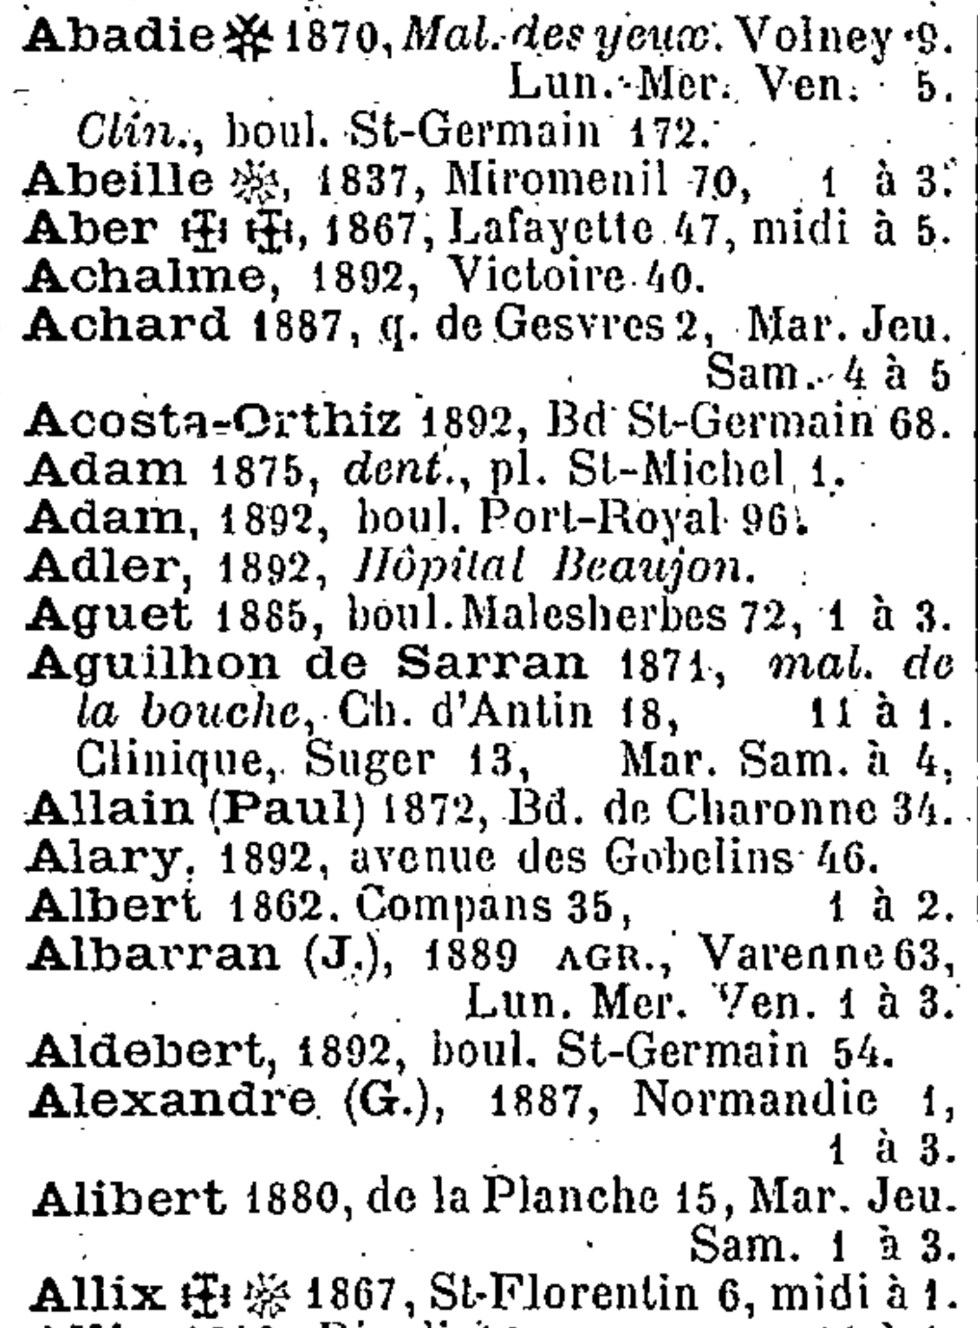
\includegraphics[width=0.4\linewidth]{Images/1893-0061.png}
    \caption{related part in 1893-0061}
    \label{fig:1893_0061_image}
\end{figure}

% \section{Conclusion and Limitation}
% From the quantitative metrics, we should use image+text or image only data sources and the Gemini 3 family models. From further qualitative studies, we showed that image only input is not stable and additional text could help with our correction. When it comes the comparison between Gemini 3 Pro Preview or Gemini 3 Flash, the metrics are close (0.01 WER difference) and two models over different files those two models still reach close results. This should be a call by budget and processing time. Enough time and money, go pro. Otherwise, flash won't be very far behind. \textbf{In our actual extraction for the selected 4,166 pages dataset, we use Gemini 3 Pro Preview and Image + Text (Original OCR) input}. Section~\ref{sec:female} shows an initial analysis for the extracted female doctors.

% Global metrics are vague, hiding more finegrained results. Qualitative studies are case based. Different cases may result in different results, but analyse time is limited. The benchmark itself isn't always correct (phu in Table~\ref{tab:qualitative_model_comparison} example 2), although we tried our best.

\section{Conclusion and Limitations}

Based on the quantitative metrics, the optimal configurations are either \textit{image-only} or \textit{image+text} inputs combined with models from the Gemini~3 family. Further qualitative analysis shows that \textit{image-only} inputs can be unstable in certain cases, while the addition of textual input helps correct ambiguities and improves robustness.

When comparing Gemini~3 Pro Preview and Gemini~3 Flash, the performance gap is minimal, with an average difference of about 0.01 in WER. Across different subsets of files, both models yield highly comparable results. As such, the choice between the two should primarily depend on budget constraints and processing-time requirements: when resources allow, Gemini~3 Pro Preview is preferable; otherwise, Gemini~3 Flash remains a strong and reliable alternative. \textbf{For the final extraction of the selected dataset comprising 4,166 pages, we adopted Gemini~3 Pro Preview with an Image+Text (original OCR) input configuration}. Section~\ref{sec:female} presents an initial analysis of the extracted female physicians.

Several limitations should be noted. Global metrics tend to obscure more fine-grained behaviors, while qualitative analyses are inherently case-based and cannot exhaustively cover all error patterns within a limited analysis time. Moreover, the benchmark itself is not always error-free (e.g., the ``phu'' case in Table~\ref{tab:qualitative_model_comparison}, Example~2), despite our efforts to verify and clean the reference data.